\chapter{Летописи продолжают}

Продолжим изучать летописные сведения о Городке. Возможно, в разные годы поселение с таким названием находилось в разных местностях. Такое впечатление у меня порой складывается при сравнении записей из летописей. 

Однако ничего вернее сказанного в предыдущей главе вычислить не получается. Я уверен в том, что на 1110 год, урочище (скажем так) Радосынь совпадало с местом, которое ныне занимает озеро Радусен на окраине Погребов. На какое пространство распространялось название Радосыни, я не знаю. На девяносто процентов я уверен в правильности предположения, что Городец 1110 года стоял на Сторожевых горах у Погребов, где теперь находится ТЭЦ-6. Это мой островок надежности.  

Просто повезло, что на картах РККА подписано озеро. Остальное зыбко, и по летописям можно лишь догадываться, где был тот или иной упоминаемый Городок в таком-то году. Полистаем страницы древних списков.

За 1026 (6534) год, Ипатьевский:

\begin{quotation}
Ярослав сьвокупи воя многы и приде Кыеву, и створи мир с братом своим Мстиславом оу Городьца. и разделиста и по Днепр Рускую землю: Ярослав прия су страну, а Мъстислав ону; и начаста жити мирно и в братолюбии, и преста оусобица и мятеж и бысть тишина велика в земли Руской.
\end{quotation}

Ярослав и Мстислав заключают мир у Городка. Снова обращу внимание на особенность – не в Городке, а у Городка, то бишь возле него.

Князья разделили землю по границе, коей послужил Днепр. И зажили дружно, до поры до времени.

За 1078 (6586) год, Ипатьевский:

\begin{quotation}
Убьен бысть князь Изяслав месяца октября в 3 день, вземше тело его, привезоша в лодьи и поставиша против Городцю; и изидоша противу ему всь город Киев и, възеложиша на сане, повезоша и с песнями попове и черноризци, и понесоша в град, и не бе лзе слышати пения в плаче велике и вопле: плакася по нем весь город Киев.
\end{quotation}

Изяслава убили, согласно летописи, на «месьте на Нежатини ниве» под Черниговом. Оттуда тело князя повезли Десной в лодье к Киеву и поставили «против Городцю» – снова, почему-то не в самом Городке. Может Городец вовсе не у воды? 

На каком берегу и к берегу чего причалили лодью?

Весь город Киев вышел встречать покойника. Поместили тело на похоронные сани, «повезоша и\footnote{«и» здесь означает «его».} с песнями попове и черноризци, и понесоша в град».

Значит, тело доставили на правый берег Киева, а Городец находился где-то напротив того места, через реку.

Киев же, если уважать традиционную историю, занимал тогда Гору и Подол. Напротив лежит район Воскресенки. Возвышенность левобережной Лысой горы – хорошее место для Городка.

Однако вопрос. Ведь между левобережным «городцом» и правым берегом Днепра, лежат острова. Значит, надо предполагать, что там были не острова, но «материковая» суша, и где-то в ее глубине (возможно однако за руслом меньшей чем Днепр реки) стоял Городок, описанный в 1078 году. Вообще как давно Труханов остров – остров, а не материковая земля? А земли нынешнего острова Муромца, по земельным грамотам предстают, в 16 веке, скорее всего именно материком.

Когда при княгине Ольге, Печенеги в отсутствие Святослава осадили Киев, то войско Претича с лодьями стояло на левом берегу\footnote{Этот случай описан за 968 (6476) год, причем неясно, чей Претич был воевода, почему мялся, наблюдал, сам ничего не предпринимая до вести от ольгиного гонца. Ольга вынудила Претича подступить к осажденному правобережному Киеву, ибо Киевляне собирались сдать город Печенегам. Ольга с внуками и своими людьми (отдельно от Киевлян) хотела при помощи Претича покинуть правый берег. Хитростью Претич добился отвода войск Печенегов к Лыбеди, но сам, похоже, Ольгу так и не перевез на левый берег. Киевляне послали по Святослава, тот прибыл и прогнал Печенегов. Сочетание отсутствия Святослава в Киеве, осады Киева Печенегами, и нерешительности Претича выглядит подозрительно, будто Святослав просто подставил Ольгу, а Претич поначалу был со Святославом заодно.}, и киевский юноша-посланец переплыл туда, пробравшись из города через стан неприятеля. Но что подразумевалось под левым берегом – материк или берег большого острова?

В год 1097 (6605), в месяц «грудень, рекше ноябрь»\footnote{В современном украинском груднем обозначают 12 месяц, декабрь.} по Ипатьевской летописи, Владимир Мономах, ужаснувшись недавнему насильному ослеплению князя Василька (не буду пересказывать, эту страшную историю надо читать полностью и в подлиннике), расплакался и говорит:

\begin{quotation}
«Сего не было есть в Русьской земли ни при дедех наших, ни при отцах наших, сякого зла». 

И ту абье посла ко Давыду и к Ольгови Святославичема, глаголя: 

«поидета к Городцю, да поправим сего зла, еже ся сотвори у Руськой земли и в нас братьи, оже уверже в ны нож; да аще сего не поправим, больше зло встанет в нас, и начнет брат брата заколати, и погыбнеть земля Русьская, и врази наши Половци пришедше возьмуть землю Русьскую».
\end{quotation}

Далее Владимир и позванные им Давыд и Ольг собираются у Городка на совещание:

\begin{quotation}
Володимеру сущю с вои у бору, Володимер же, и Давы, и Олег послаша муже свои к Святополку, глаголюще: «что се створил еси в Русьской земле, уверьгл если нож в ны? чему еси ослипил брата своего? [...]»
\end{quotation}

Из этого следует, что возле Городка произрастал бор – сосновый лес. И далее:

\begin{quotation}
Наутрия же хотя Володимеру, и Давыдови, и Ольгови через Днепр на Святополка, Святополк же хотяше побегнути ис Кыева, и не даше ему Кияне побегнути [...]
\end{quotation}

Что подтверждает нахождение Городка на левом берегу, ибо Владимир Мономах хотел переправиться через Днепр к Святополку.

На следующий 1098 (6606) год, братья-князья заключают у Городка (снова не «в») мир:

\begin{quotation}
Прииде Володимер, и Давыд, и Олег на Святополка, и сташа у Городца, и створиша мир.\end{quotation}

Следующая по времени запись – за 1110 год, связана с Мономахом. Мы разобрали ее в главе про Радосынь.

За 1135 год Ипатьевский список сообщает:

\begin{quotation}
Всеволод же с братью своею [...] поидоша, воюя села и городы Переславськой власти и люди секуще, доже и до Киева придоша и Городец зажгоша на святаго Андрея день, ездяху по оной стороне Днепра, люди емлюще, а другия секуще, не утягшим перевестися им, не лзе бо бяше перевестися крами; и плениша же и скота бещисленное множество.

Ярополку бо бяше нелзе перевестися крами с своими, а они, стоявше три дни за Городцем в бору, идоша Чернигову и оттуда слюче межю собою створиша мир.
\end{quotation}

Отсюда нельзя заключить, где находился Городец.  Всеволод зажег его, да ездил по левому берегу, пленяя и убивая людей, которые не успели переправиться. Выходит, левый берег был населен. Жили в Городке или вне его, непонятно. На левом берегу также были стада, поскольку Всеволод уводит «бещисленное множество скота».

Сидящий в Киеве, на правом берегу, Ярополк не мог переправиться со своими воинами на левый. Всеволод же, постояв три дня в бору за Городком, отправился к Чернигову. А Городок, быть может, сгорел дотла и потом его отстроили на другом месте?

1146 (6654) год, Лаврентьевская летопись, про Городок молчит, зато есть Радосынь, где князь Всеволод собирает своих братьев:

\begin{quotation}
Приде Володимер и взя Прилук; и совокупи Всеволод братья свою на Радосыни, и сложи путь с Бориша дни на Володимера, и начере оба Изяслава оставити дома; и перебы неколико, и разболеся велми, и везоша и Вышегороду, и тамо скончася месяца июля в 30 день.
\end{quotation}

Далее, снова Ипатьевская летопись, 1151 год, знаменитая попытка переправы Гюрги (Юрия Долгорукого) через Днепр к Киеву. Перед тем, как Гюрги из Городка Остёрского, по рекам Остёр и Десна прибыл к Родуни, произошла такая расстановка сил:

\begin{quotation}
Тогда же Изяслав Давыдович иде Киеву к Вячьславу и к Изяславу Мстиславичу, и сташа у Городка, и ту створиша Георгев день.
\end{quotation}

Изяслав Давыдович в Георгиев день сташа у Городка. Это Городок Киевский, не Остёрский. А тот ли это Городок, что в предыдущих записях летописи – бог весть.

%Сорок лет прошло, крепость могла переместиться – старая оставлена, новая построена, или же прежнюю никто не трогал, но срубили еще одну? А слово «городок», кажись, было тогда столь же привычным, как например «слобода».

Любопытно – Изяслав стал не «в» Городке, а «у» Городка. Может потому, что передвигался по воде в насадах, а может это проявление отмеченной мною странности. Будто есть какой-то Городок, но туда не заходят.

Прочтем, что случилось далее: 

\begin{quotation}
И поиде Гюрги к Киеву и сташа в Родуни, и придоша Половци диции мнози Дюргеви в помочь;
\end{quotation}

Гюрги идет к Киеву (по Десне, в лодьях) и останавливается в Родуни, а по суше подходит подмога – дикие Половцы.

Но Изяслав стоит «у Городка». На каком это расстоянии от Родуни? Сейчас я не задаю вопрос о тождественности Родуни и Радосыни. Есть два противника в двух точках на местности – Изяслав у Городка, и Гюрги в Родуни.

Очевидно, между ними должно быть какое-то расстояние, достаточное, чтобы не началось сражение, потому что Гюрги в Родуни еще подождал Половцев.

Предположу что Изяслав «у Городка» оттуда не мог видеть, что происходит в Родуни. Но летопись дает второй ориентир нахождения Изяслава: 

\begin{quotation}
и Изяславу же блюдущу вбрести в Днепр,
\end{quotation}

Изяслав охранял брод через Днепр – где могли бы переправиться Половцы. Этот брод был возле устья Десны, ибо далее воины Изяслава в насадах начинают сражаться на воде с лодьями Гюрги, на протяженности от Киева до устья Десны:

\begin{quotation}
и тако начаша ся бити по Днепру у насадех от Кыева оли и до устья Десны, ови ис Киева в насадех выездяху биться, а они ис товар; и тако бьяхутся крепко, не могоша бо что успети противу Киеву. 
\end{quotation}

Значит, Изяслав, будучи в насадах «у Городка» (дополнительные насады выплывали из Киева), сторожил устье Десны. И ничего у Гюрги не получилось.

Но разве мы знаем, где тогда было устье Десны?

В более чем двухсотстраничной «Пояснительной записке к проекту окончания выправительных работ на р. Днепре у г. Киева» инженера Николая Максимовича, изданной в Киеве в 1896 году, я наткнулся на странное сообщение:

\begin{quotation}
На выкопированных нами старинных планах города Киева можно также найти разные указания на изменчивость русла реки Днепра и его рукавов под городом Киевом.

Так, на плане XI века устье реки Десны показано впадающим в Днепр всего в 3-х верстах выше города Киева (ныне Десна впадает в 10 верстах выше). В настоящее время в этом приблизительно пункте находится впадение рукава Десенки в рукав Черторой.
\end{quotation}

Сомневаюсь, чтобы Максимович нашел где-то план 11 века, хотя чем черт не шутит? Однако, вероятно, Максимович таки перерисовал некую старинную карту с таким положением дел, жаль только не приводит ее в своей «Записке» и непонятно, как именно протекала Десна до своего устья. 

Однако важно указание на место этого давнего устья Десны в переложении на конец 19 века – «впадение рукава Десенки в рукав Черторой». Это широта северной части Воскресенки. Почти широта Алмазного озера, этой части былого русла Десны. Где-то именно там она и должна была выруливать к Днепру!

Подтверждение этому я нашел, внимательно прочитав «Книгу большому чертежу»\cite{chert} - словесному описанию карты Российской империи, составленному в 1627 году. Она гласит: «А ниже Десны реки в полтретьи версты на Днепре с Литовской стороны на правом берегу город Киев», и в списке: «а ниже устья реки Остря 60 верст река Десна пала в Днепр, выше города Киева 2 1/2 версты». Это 2,5 версты - почти точное расстояние от Подола до той же широты смычки Воскресенки с Выгуровщиной.

А вот на карте всего Днепра, составленной де Боскетом в 1742 году, Десна впадает в Днепр южнее Хотяновки и севернее Осещины. С юга на север – Троещина, на той же части материка – Осещина, затем устье Десны, и выше – Хотяновка. Сейчас же устье Десны – южнее Осещины. При устье показан большой остров, а на правом берегу Днепра, почти напротив – Выш Городок, там где ныне Вышгород.

\begin{center}
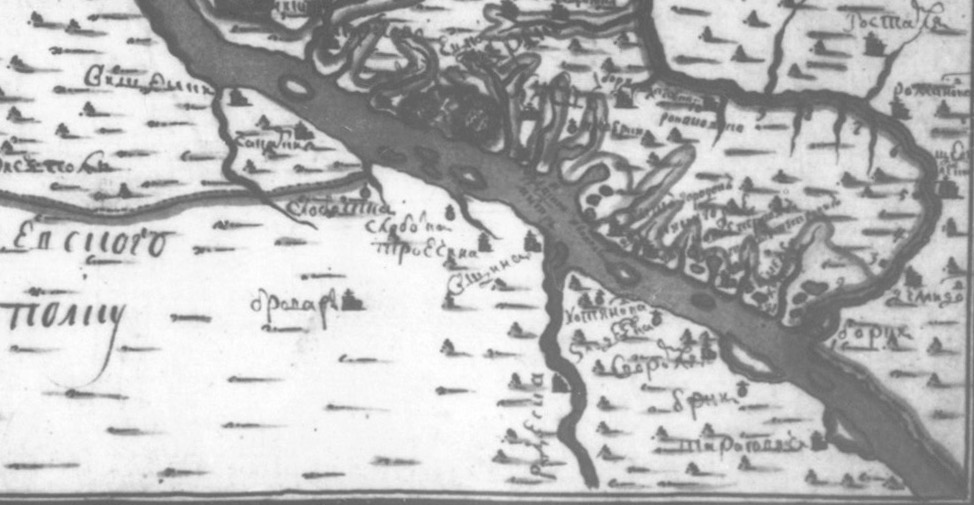
\includegraphics[width=\linewidth]{chast-gorodki/letopisi/1742-de_bosket.jpg}

\textit{Кусок плана 1742 года.}
\end{center}

Как понимаю, некогда существовало два устья Десны – в разное ли время два, либо два сразу в некоторое время, а потом осталось одно. 

Южное устье, от «Алмазного» русла – древнее. Северное – кажется более новое, однако довольно резво смещавшееся к севера на юг. Движение устья не всегда означает физическое перемещение конца русла. Нет, просто один рукав отмирает, другой набирает силу, и устьем считается конец уже этого другого рукава.

Вернемся к летописи! Гюрги с союзниками, не сумев переправиться на правый берег, проскочил до Труханова острова, к озеру Дулебскому.

А как? Просто мимо Подола? За какими-то островами? Каков тогда вообще был рельеф местности? Вдруг устье Десны было на широте Подола и Воскресенки?

Где же находился Городок, упомянутый в 1151 году – там ли, где в 1110 году, или в другом месте? Родунь ли Радосынь? В этих соседних по упоминанию Городка летописных записях есть отсылка к похожим (однако без указания на тождественность) названиям – Радосынь и Родунь. Ни до, ни после 1110 и 1151 года, Городок с ними не связан.

Еще одно замечание – в описании перемещений Гюрги в пределах Киева в 1151-м используются названия только трех урочищ – устье Десны, Днепр, Родунь и Городец. Никакой Черторыи и Радосыни.

Прикидывая, где что могло быть, я нарисовал для себя по карте РККА схему. Разумеется осозна\'ю, что на ней совершенно иной рельеф, чем в летописные времена, но мне нужна какая-то основа, да и сама эта карта очень нравится.

\begin{center}
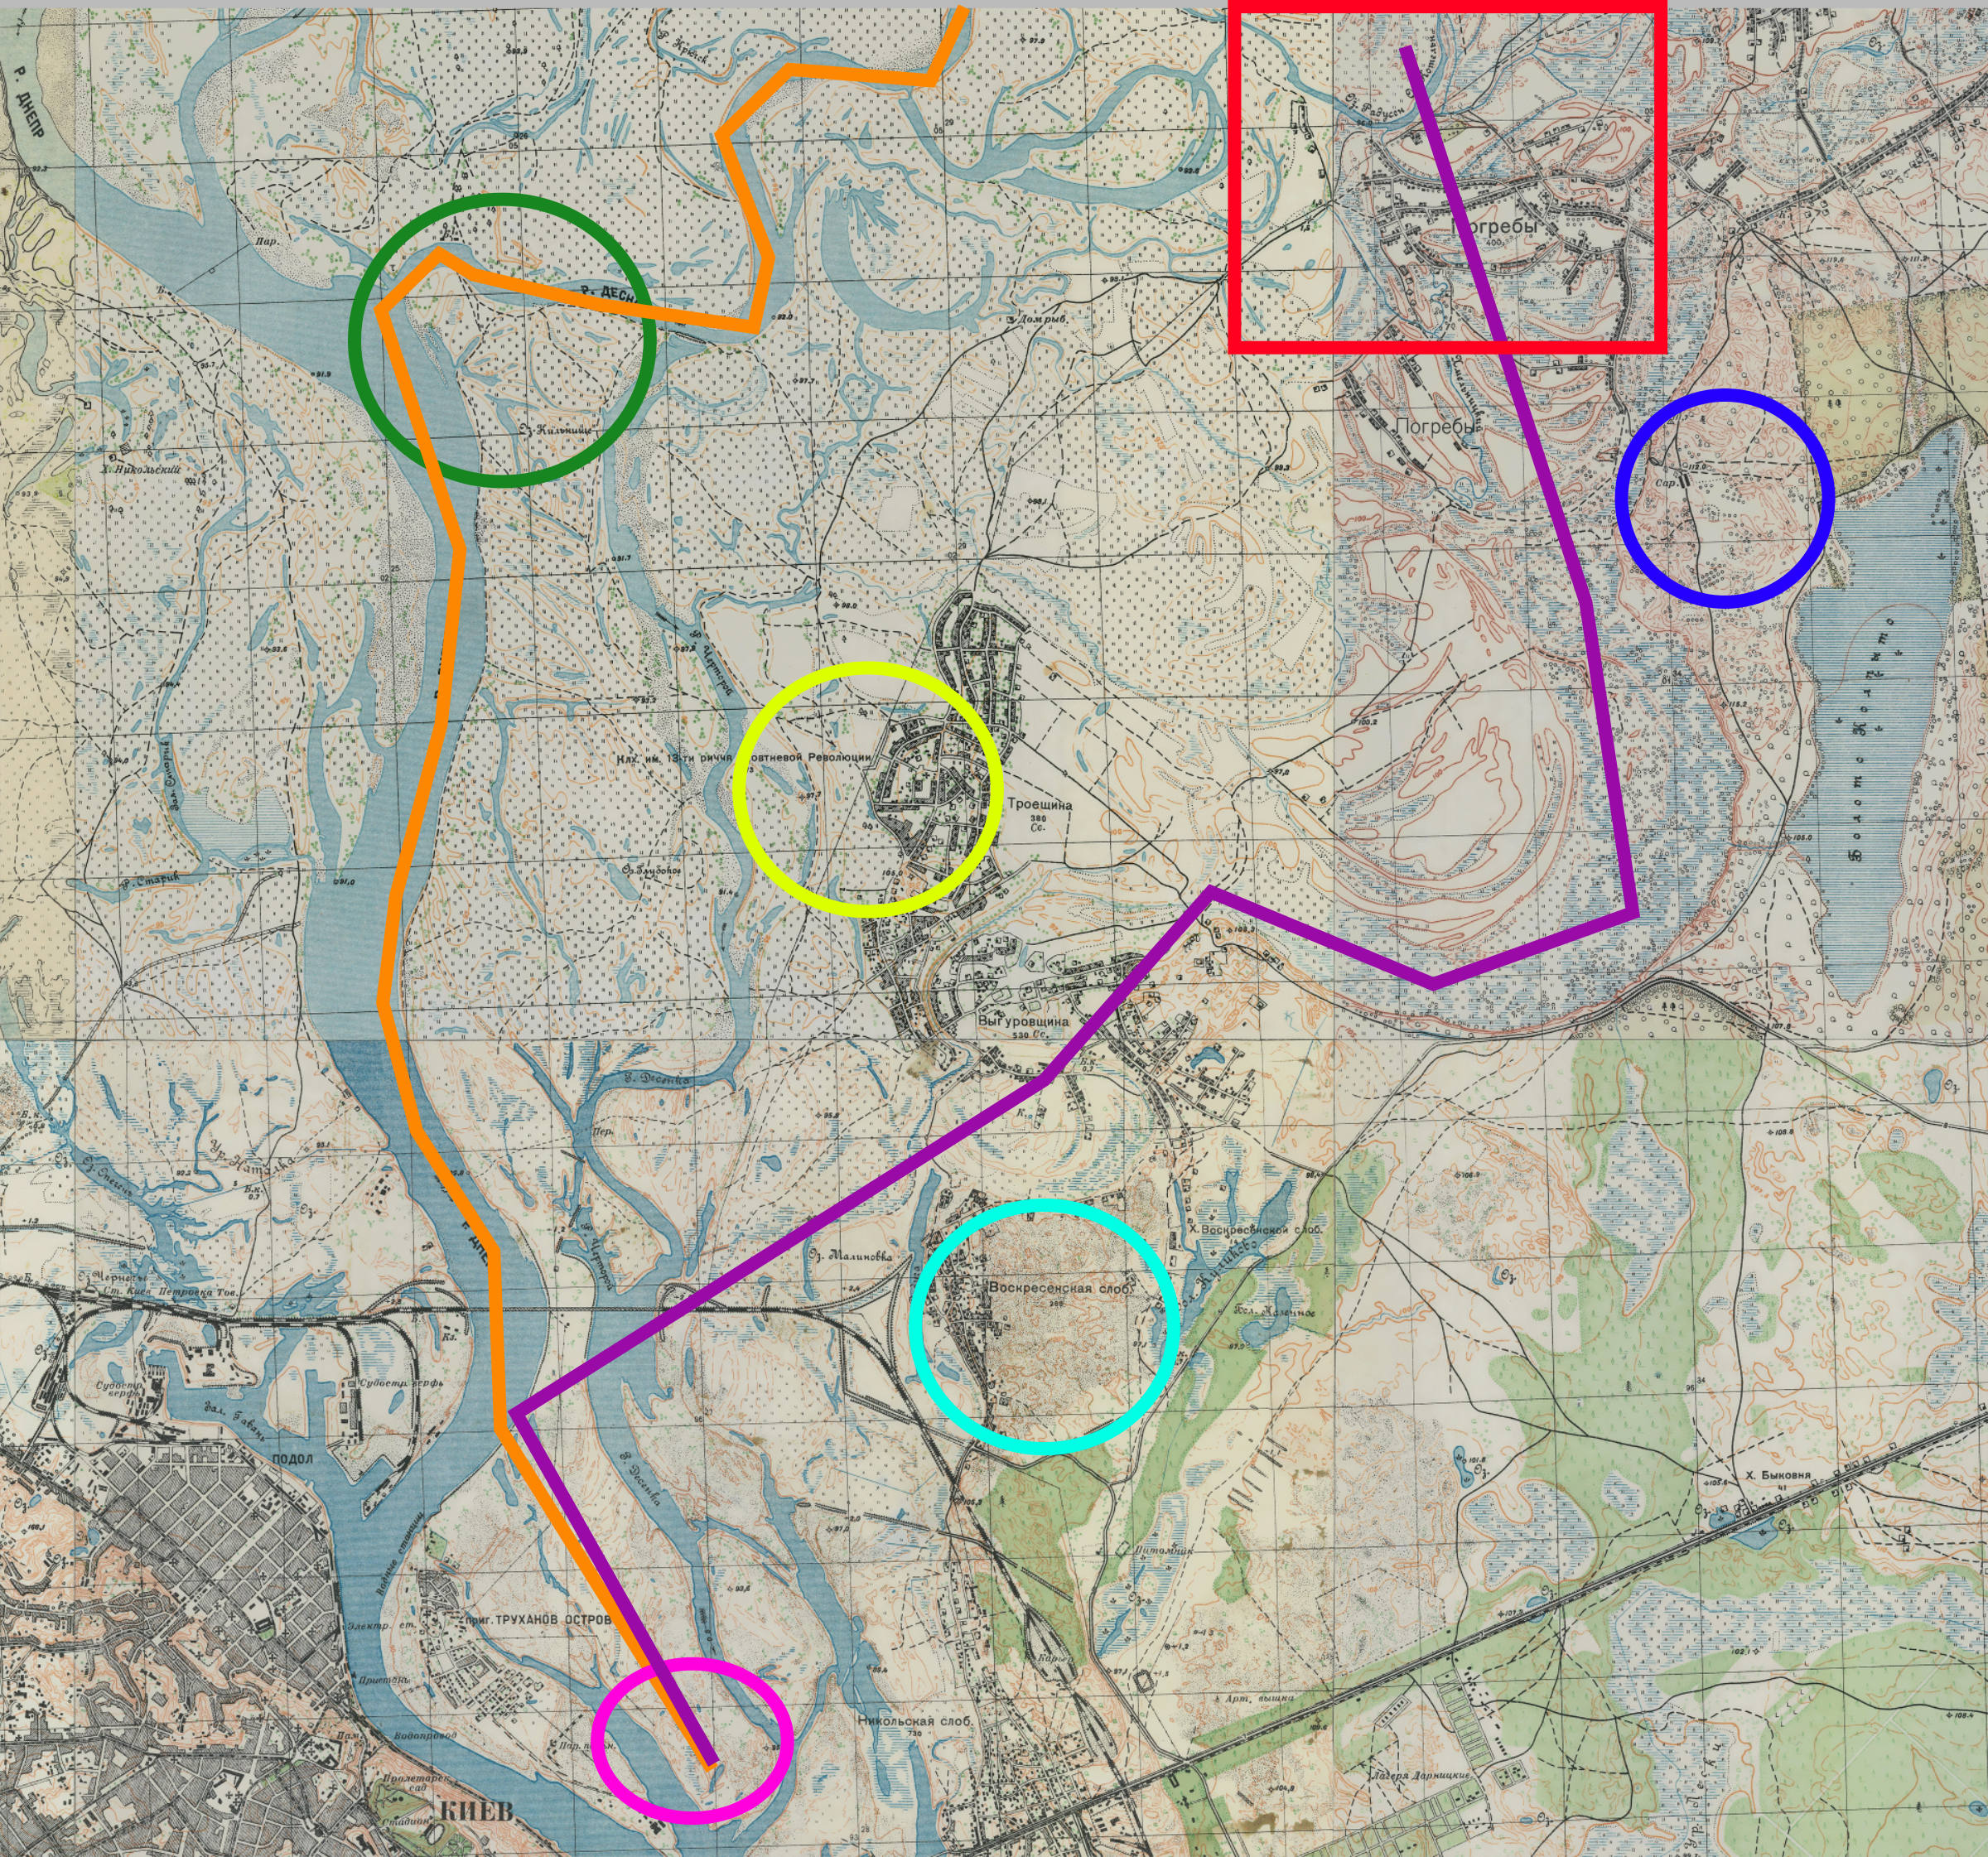
\includegraphics[width=\linewidth]{chast-gorodki/letopisi/gurgi-dvij.jpg}
\end{center}

Теперь расскажу, что нарисовал. 

Красным квадратом я выделил единственное, в чем уверен – место нахождения Радосыни в 1110 году. Синий круг – там, на горе с нынешней ТЭЦ-6, предполагаю Городок 1110 года.

Малиновый круг – Долобське, куда Гюрги на лодьях добрался из Родуни по Днепру.

Зеленый круг – устье Десны в 1930-х годах, и все привыкли считать, что это устье веками с летописных времен сохраняется примерно по этой широте. Если Городок в 1151 году был где-то там, на роль его остатков подходит городище на острове Муромце.

Желтый круг – возле Гнилуши у Выгуровщины ученые полагают Городок, а заодно – позже – замок (укрепленный двор) князя Олельковича.

Бирюзовый круг – где мог быть Городок (не тот, что в 1110 году) на Воскресенке.

Оранжевая линия – как бы двигался Гюрги из некой Родуни, если б в 1151 году Десна и Днепр имели современные русла. При этом, по летописи, на протяженности от зеленого круга до малинового шло сражение на воде.

Фиолетовая линия – как бы двигался Гюрги из Родуни, если бы она была Радосынью, а Десна протекала по своему прежнему (древнему?) руслу, остатки которого прослеживаются по цепи болот и ложбин. В таком случае устье Десны могло находиться напротив Подола. Сюда также вписывается Городок на Воскресенке. В самом деле, если Изяслав – «у Городка», и одновременно с этим сторожит переправу через Днепр, а битва происходит по Днепру от Киева до устья Десны, то если устье Десны на уровне Подола, то Городок на Воскресенке предшествует устью. Можно даже вообразить, что Десна протекала и по современному руслу озера Радунки.

В 6745 (1237) году Городок в последний раз появляется на страницах Ипатьевской летописи, где повествуется о пришествии Татар под Киев:

\begin{quotation}
Меньгуканови же пришедшу сглядать град Кыева, ставшу же ему на оной стране Днепра во градка Песочного, видив град удивися красоте его и величеству его.
\end{quotation}

Градок Песочный – значит, стоит среди песков. На ум приходит цепь песочных дюн левобережной Лысой горы.

Снова непонятно, Городок Песочный – это Городок из какого-либо прежнего летописного сообщения, или другой Городок, потому и о нем уточнено, чтобы отделить от прочих – Песочный.

Меньгукан – кан, хан Меньгу (ученые почему-то переиначили слово «кан» с «хан») стал «во Градка» – а по Хлебниковскому списку «у Градка». Оттуда он «сглядал Киев», высматривал или обозревал его, и видя оный, удивлялся красоте и величеству его.

Откуда же видно Киев? Предположим, речь идет о Киеве как о Горе и Подоле. Еще в конце 19 века ученый Гошкевич, а следом за ним Петров, повторяли, что Меньгукан остановился в Городке около озера Гнилуши, и оттуда глядел на Киев.

Гошкевич в своем докладе «Замок князя Симеона Олельковича и летописный городок под Киевом», читанном 18 сентября 1889 года, писал:

\begin{quotation}
В весеннее же половодье вся равнина от Киева, через остров Муромец, и Черниговское побережье, вплоть до левого берега Гнилуши, представляет сплошное водное пространство, на берегу которого высятся валы Городка\footnote{Высоту валов Гошкевич определяет в 2 сажени – несколько более 4 метров.}. [...]

Сидя на валах древнего городища, мы любовались чудной панорамой Киева, открывающеюся перед нашими глазами. Город виден решительно весь: от Приорки до Выдубицкого монастыря. Подернутые легкой дымкой налегшего на землю тумана, обрисовывались силуэты церквей и домов; Киев утопал в зелени, еще не увядшей под дыханием осени.
\end{quotation}

Я смотрел с берега Гнилуши, в самом ли деле Меньгукан мог «сглядать» с возвышенного берега весь Киев. Так вот, с того пригорка я видел Московский мост, Приорку, телебашню, однако Подол и южнее были заслонены от меня деревьями.

Даже с более высокой точки на улице Деснянской  – что севернее Гнилуши, тоже всё заслоняют деревья. Не думаю, что в конце 19 века пространство было голым и пустынным. По левому берегу в низовьях Воскресенки темнел сосновый лес, местность Труханова и нынешнего Гидропарка кудрявилась слободскими садами. А Выдубичи даже теоретически не просматриваются.
